\section{Experiments}

The highest F1 score we found came from the following process in the fully automated pipeline: for every trial generated by the Optuna study, we construct the encoder and, when enabled, a decoder for autoencoder-based models, apply He initialization, train over all $K$ folds using PyTorch Lightning, perform model-level windowing, and aggregate predictions.

The best model is chosen using the macro-averaged F1 score, a metric particularly suitable for class-imbalanced multiclass problems as in our case.

$
\text{F1}_{\text{macro}} = \frac{1}{C} \sum_{c=1}^{C} \text{F1}_c,
\text{F1}_c = \frac{2 \,\text{Precision}_c \,\text{Recall}_c}{\text{Precision}_c + \text{Recall}_c}.
$

\begin{figure}[H]
    \centering
    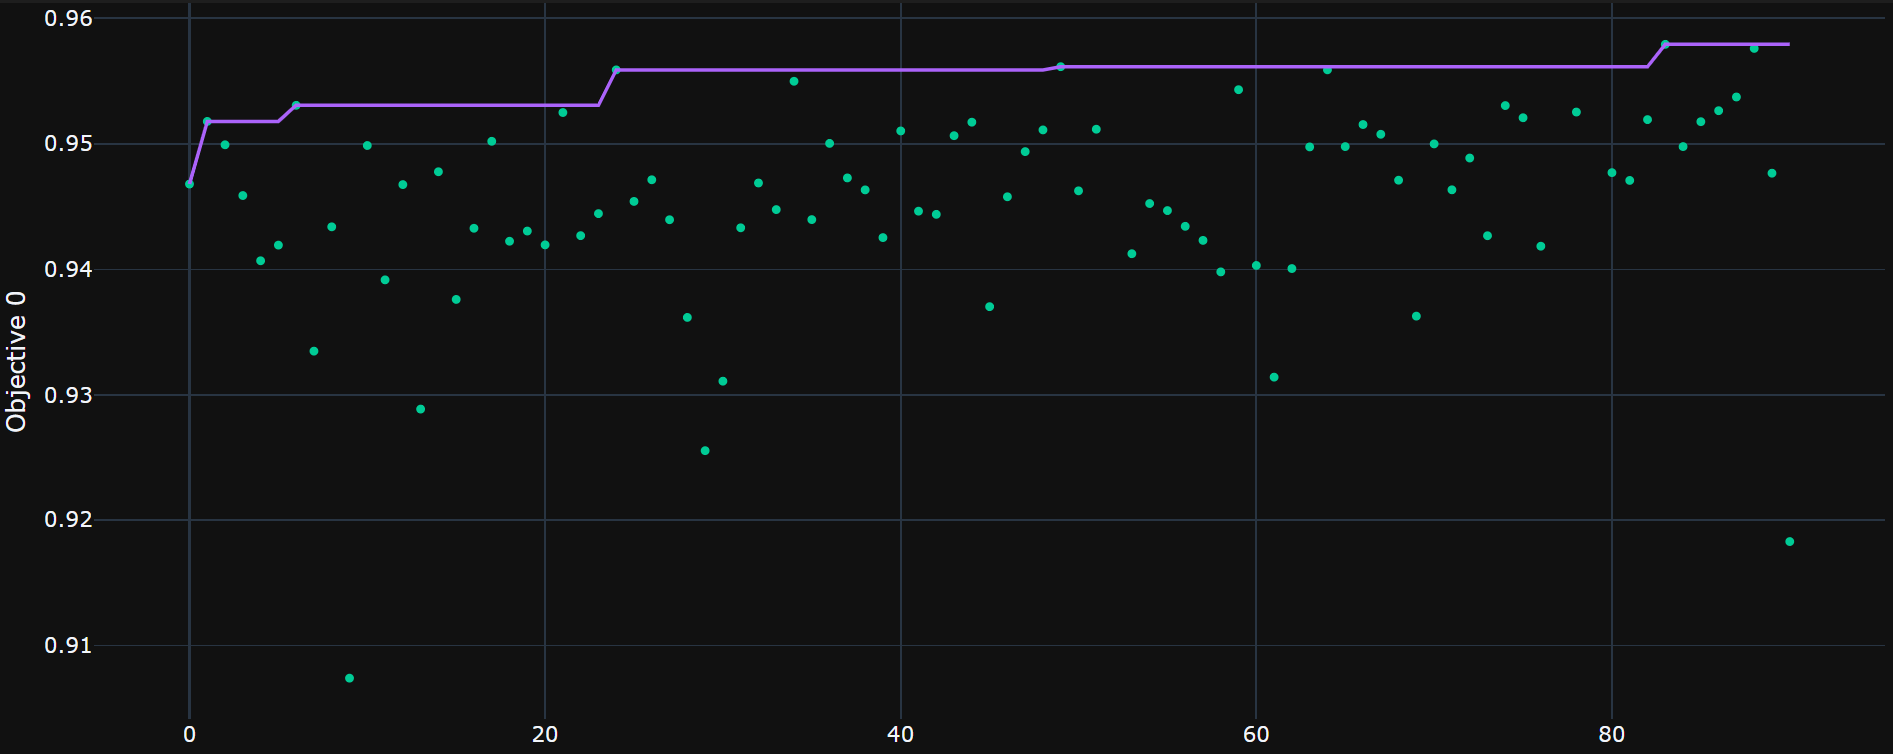
\includegraphics[width=\linewidth]{Deliverables/Report1/img/optuna.png}
    \label{fig:Optuna}
\end{figure}


%Additionally, during development we monitored also validation loss, per-class precision and recall, training/validation time per fold, and the number of parameters and computational cost of each model.
